\chapter{مرتب‌سازی}

\index{مرتب‌سازی}

\key{مرتب‌سازی}
مسئله‌ای بنیادین در طراحی الگوریتم است.
بسیاری از الگوریتم‌های کارآمد
از مرتب‌سازی به عنوان یک زیرروال استفاده می‌کنند،
زیرا پردازش داده‌ها در صورتی که عناصر مرتب باشند،
اغلب آسان‌تر است.

به عنوان مثال، مسئله «آیا آرایه شامل دو عنصر برابر است؟»
با استفاده از مرتب‌سازی به سادگی حل می‌شود.
اگر آرایه شامل دو عنصر برابر باشد،
آن‌ها پس از مرتب‌سازی کنار یکدیگر قرار می‌گیرند،
بنابراین یافتن آن‌ها آسان است.
همچنین مسئله «پرتکرارترین عنصر در یک آرایه چیست؟»
را می‌توان به شیوه مشابهی حل کرد.

الگوریتم‌های زیادی برای مرتب‌سازی وجود دارد و آن‌ها
نمونه‌های خوبی برای چگونگی به‌کارگیری تکنیک‌های مختلف
طراحی الگوریتم هستند.
الگوریتم‌های عمومی و کارآمد مرتب‌سازی
در زمان $O(n \log n)$ عمل می‌کنند،
و بسیاری از الگوریتم‌هایی که از مرتب‌سازی به عنوان زیرروال
استفاده می‌کنند نیز همین پیچیدگی زمانی را دارند.

\section{نظریه مرتب‌سازی}

مسئله پایه‌ای در مرتب‌سازی به شرح زیر است:
\begin{framed}
\noindent
آرایه‌ای شامل $n$ عنصر به شما داده شده است،
وظیفه شما مرتب‌سازی عناصر به ترتیب صعودی است.
\end{framed}
\noindent
به عنوان مثال، آرایه
\begin{center}
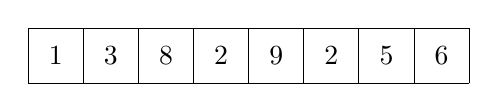
\begin{tikzpicture}[scale=0.7]
\draw (0,0) grid (8,1);
\node at (0.5,0.5) {$1$};
\node at (1.5,0.5) {$3$};
\node at (2.5,0.5) {$8$};
\node at (3.5,0.5) {$2$};
\node at (4.5,0.5) {$9$};
\node at (5.5,0.5) {$2$};
\node at (6.5,0.5) {$5$};
\node at (7.5,0.5) {$6$};
\end{tikzpicture}
\end{center}
پس از مرتب‌سازی به صورت زیر درخواهد آمد:
\begin{center}
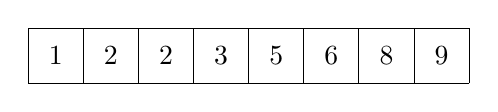
\begin{tikzpicture}[scale=0.7]
\draw (0,0) grid (8,1);
\node at (0.5,0.5) {$1$};
\node at (1.5,0.5) {$2$};
\node at (2.5,0.5) {$2$};
\node at (3.5,0.5) {$3$};
\node at (4.5,0.5) {$5$};
\node at (5.5,0.5) {$6$};
\node at (6.5,0.5) {$8$};
\node at (7.5,0.5) {$9$};
\end{tikzpicture}
\end{center}

\subsubsection{الگوریتم‌های $O(n^2)$}

\index{مرتب‌سازی حبابی}

الگوریتم‌های ساده مرتب‌سازی آرایه
در زمان $O(n^2)$ اجرا می‌شوند.
چنین الگوریتم‌هایی کوتاه هستند و معمولا
از دو حلقه تو در تو تشکیل می‌شوند.
یک الگوریتم معروف مرتب‌سازی با زمان $O(n^2)$،
\key{مرتب‌سازی حبابی} است که در آن عناصر
با توجه به مقادیرشان در آرایه «حباب» می‌زنند و بالا می‌آیند.

مرتب‌سازی حبابی از $n$ دور تشکیل شده است.
در هر دور، الگوریتم در میان عناصر آرایه پیمایش می‌کند.
هر زمان که دو عنصر متوالی با ترتیب نادرست یافت شوند،
الگوریتم جای آن‌ها را عوض می‌کند.
الگوریتم را می‌توان به صورت زیر پیاده‌سازی کرد:
\begin{lstlisting}
for (int i = 0; i < n; i++) {
    for (int j = 0; j < n-1; j++) {
        if (array[j] > array[j+1]) {
            swap(array[j],array[j+1]);
        }
    }
}
\end{lstlisting}

پس از دور اول الگوریتم،
بزرگ‌ترین عنصر در جایگاه صحیح قرار خواهد گرفت،
و به طور کلی پس از $k$ دور، $k$ عنصر بزرگ‌تر
در جایگاه‌های صحیح خواهند بود.
بنابراین پس از $n$ دور، کل آرایه مرتب خواهد شد.

به عنوان مثال، در آرایه

\begin{center}
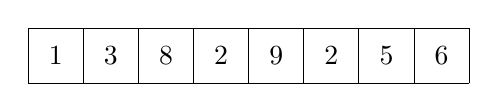
\begin{tikzpicture}[scale=0.7]
\draw (0,0) grid (8,1);

\node at (0.5,0.5) {$1$};
\node at (1.5,0.5) {$3$};
\node at (2.5,0.5) {$8$};
\node at (3.5,0.5) {$2$};
\node at (4.5,0.5) {$9$};
\node at (5.5,0.5) {$2$};
\node at (6.5,0.5) {$5$};
\node at (7.5,0.5) {$6$};
\end{tikzpicture}
\end{center}

\noindent
دور نخست مرتب‌سازی حبابی عنصرها را به این ترتیب جابه‌جا می‌کند:

\begin{center}
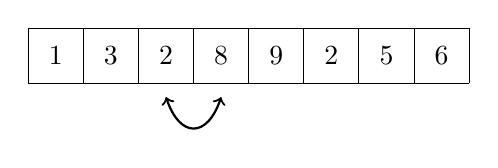
\begin{tikzpicture}[scale=0.7]
\draw (0,0) grid (8,1);
\node at (0.5,0.5) {$1$};
\node at (1.5,0.5) {$3$};
\node at (2.5,0.5) {$2$};
\node at (3.5,0.5) {$8$};
\node at (4.5,0.5) {$9$};
\node at (5.5,0.5) {$2$};
\node at (6.5,0.5) {$5$};
\node at (7.5,0.5) {$6$};

\draw[thick,<->] (3.5,-0.25) .. controls (3.25,-1.00) and (2.75,-1.00) .. (2.5,-0.25);
\end{tikzpicture}
\end{center}

\begin{center}
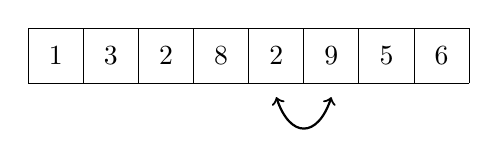
\begin{tikzpicture}[scale=0.7]
\draw (0,0) grid (8,1);
\node at (0.5,0.5) {$1$};
\node at (1.5,0.5) {$3$};
\node at (2.5,0.5) {$2$};
\node at (3.5,0.5) {$8$};
\node at (4.5,0.5) {$2$};
\node at (5.5,0.5) {$9$};
\node at (6.5,0.5) {$5$};
\node at (7.5,0.5) {$6$};

\draw[thick,<->] (5.5,-0.25) .. controls (5.25,-1.00) and (4.75,-1.00) .. (4.5,-0.25);
\end{tikzpicture}
\end{center}

\begin{center}
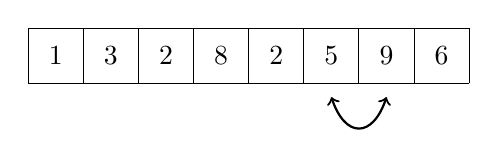
\begin{tikzpicture}[scale=0.7]
\draw (0,0) grid (8,1);
\node at (0.5,0.5) {$1$};
\node at (1.5,0.5) {$3$};
\node at (2.5,0.5) {$2$};
\node at (3.5,0.5) {$8$};
\node at (4.5,0.5) {$2$};
\node at (5.5,0.5) {$5$};
\node at (6.5,0.5) {$9$};
\node at (7.5,0.5) {$6$};

\draw[thick,<->] (6.5,-0.25) .. controls (6.25,-1.00) and (5.75,-1.00) .. (5.5,-0.25);
\end{tikzpicture}
\end{center}

\begin{center}
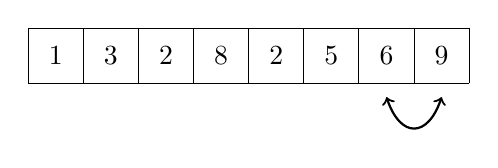
\begin{tikzpicture}[scale=0.7]
\draw (0,0) grid (8,1);
\node at (0.5,0.5) {$1$};
\node at (1.5,0.5) {$3$};
\node at (2.5,0.5) {$2$};
\node at (3.5,0.5) {$8$};
\node at (4.5,0.5) {$2$};
\node at (5.5,0.5) {$5$};
\node at (6.5,0.5) {$6$};
\node at (7.5,0.5) {$9$};

\draw[thick,<->] (7.5,-0.25) .. controls (7.25,-1.00) and (6.75,-1.00) .. (6.5,-0.25);
\end{tikzpicture}
\end{center}

\subsubsection{وارونگی‌ها}

\index{وارونگی}

مرتب‌سازی حبابی نمونه‌ای از الگوریتم مرتب‌سازی است که همواره عنصرهای \emph{مجاور} در آرایه را جابه‌جا می‌کند.
مشخص می‌شود پیچیدگی زمانی چنین الگوریتمی \emph{همواره} حداقل $O(n^2)$ است، زیرا در بدترین حالت، $O(n^2)$ جابه‌جایی برای مرتب‌سازی آرایه نیاز است.

یک مفهوم کاربردی در تحلیل الگوریتم‌های مرتب‌سازی،
\key{وارونگی} (inversion) است:
جفتی از عناصر آرایه
$(\texttt{array}[a],\texttt{array}[b])$ به‌طوری که
$a<b$ و $\texttt{array}[a]>\texttt{array}[b]$ باشد؛
یعنی عناصر ترتیب نادرست دارند.
برای نمونه، آرایه
\begin{center}
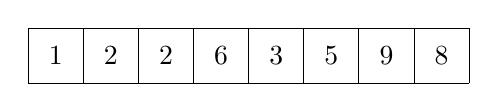
\begin{tikzpicture}[scale=0.7]
\draw (0,0) grid (8,1);
\node at (0.5,0.5) {$1$};
\node at (1.5,0.5) {$2$};
\node at (2.5,0.5) {$2$};
\node at (3.5,0.5) {$6$};
\node at (4.5,0.5) {$3$};
\node at (5.5,0.5) {$5$};
\node at (6.5,0.5) {$9$};
\node at (7.5,0.5) {$8$};
\end{tikzpicture}
\end{center}
سه وارونگی دارد: $(6,3)$، $(6,5)$ و $(9,8)$.
تعداد وارونگی‌ها نشان می‌دهد
مرتب‌سازی آرایه چقدر کار نیاز دارد.
آرایه زمانی کاملاً مرتب است که
هیچ وارونگی وجود نداشته باشد.
از طرف دیگر، اگر عناصر آرایه
ترتیب معکوس داشته باشند،
تعداد وارونگی‌ها بیشترین مقدار ممکن است:
\[1+2+\cdots+(n-1)=\frac{n(n-1)}{2} = O(n^2)\]

جابه‌جایی یک جفت عنصر متوالی با ترتیب نادرست،
دقیقاً یک وارونگی از آرایه کم می‌کند.
بنابراین، اگر الگوریتم مرتب‌سازی فقط بتواند
عناصر متوالی را جابه‌جا کند، هر جابه‌جایی حداکثر
یک وارونگی حذف می‌کند و پیچیدگی زمانی
الگوریتم حداقل $O(n^2)$ است.

\subsubsection{الگوریتم‌های $O(n \log n)$}

\index{مرتب‌سازی ادغامی}

مرتب‌سازی کارآمد آرایه در زمان $O(n \log n)$
با الگوریتم‌هایی ممکن است که به جابه‌جایی عناصر متوالی محدود نیستند.
یکی از این الگوریتم‌ها \key{مرتب‌سازی ادغامی}\footnote{بر اساس \cite{knu983}،
مرتب‌سازی ادغامی در سال ۱۹۴۵ توسط جان فون نویمان ابداع شد.}
است که بر پایه بازگشت کار می‌کند.

مرتب‌سازی ادغامی، زیرآرایه \texttt{array}$[a \ldots b]$ را به این شکل مرتب می‌کند:

\begin{enumerate}
\item اگر $a=b$ باشد، کاری انجام ندهید، زیرا زیرآرایه از قبل مرتب است.
\item موقعیت عنصر میانی را محاسبه کنید: $k=\lfloor (a+b)/2 \rfloor$.
\item زیرآرایه \texttt{array}$[a \ldots k]$ را بازگشتی مرتب کنید.
\item زیرآرایه \texttt{array}$[k+1 \ldots b]$ را بازگشتی مرتب کنید.
\item زیرآرایه‌های مرتب‌شده \texttt{array}$[a \ldots k]$ و
\texttt{array}$[k+1 \ldots b]$ را در زیرآرایه مرتب‌شده \texttt{array}$[a \ldots b]$
\emph{ادغام} کنید.
\end{enumerate}

مرتب‌سازی ادغامی کارآمد است، زیرا
طول زیرآرایه را در هر مرحله نصف می‌کند.
بازگشت شامل $O(\log n)$ سطح است
و پردازش هر سطح به زمان $O(n)$ نیاز دارد.
ادغام زیرآرایه‌های \texttt{array}$[a \ldots k]$ و \texttt{array}$[k+1 \ldots b]$
در زمان خطی ممکن است، زیرا از قبل مرتب هستند.

برای نمونه، مرتب‌سازی آرایه زیر را در نظر بگیرید:
\begin{center}
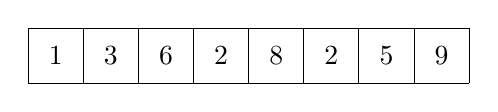
\begin{tikzpicture}[scale=0.7]
\draw (0,0) grid (8,1);
\node at (0.5,0.5) {$1$};
\node at (1.5,0.5) {$3$};
\node at (2.5,0.5) {$6$};
\node at (3.5,0.5) {$2$};
\node at (4.5,0.5) {$8$};
\node at (5.5,0.5) {$2$};
\node at (6.5,0.5) {$5$};
\node at (7.5,0.5) {$9$};
\end{tikzpicture}
\end{center}

آرایه به صورت زیر به دو زیرآرایه تقسیم می‌شود:
\begin{center}
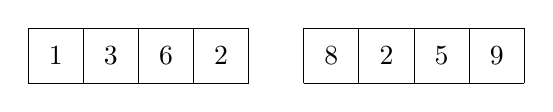
\begin{tikzpicture}[scale=0.7]
\draw (0,0) grid (4,1);
\draw (5,0) grid (9,1);

\node at (0.5,0.5) {$1$};
\node at (1.5,0.5) {$3$};
\node at (2.5,0.5) {$6$};
\node at (3.5,0.5) {$2$};

\node at (5.5,0.5) {$8$};
\node at (6.5,0.5) {$2$};
\node at (7.5,0.5) {$5$};
\node at (8.5,0.5) {$9$};
\end{tikzpicture}
\end{center}

سپس، زیرآرایه‌ها به صورت بازگشتی به این شکل مرتب می‌شوند:
\begin{center}
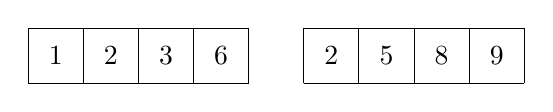
\begin{tikzpicture}[scale=0.7]
\draw (0,0) grid (4,1);
\draw (5,0) grid (9,1);

\node at (0.5,0.5) {$1$};
\node at (1.5,0.5) {$2$};
\node at (2.5,0.5) {$3$};
\node at (3.5,0.5) {$6$};

\node at (5.5,0.5) {$2$};
\node at (6.5,0.5) {$5$};
\node at (7.5,0.5) {$8$};
\node at (8.5,0.5) {$9$};
\end{tikzpicture}
\end{center}

در نهایت، الگوریتم زیرآرایه‌های مرتب‌شده را ادغام کرده و آرایه مرتب‌شده نهایی را تولید می‌کند:
\begin{center}
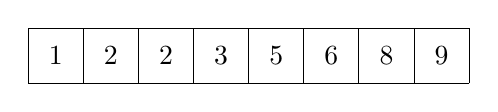
\begin{tikzpicture}[scale=0.7]
\draw (0,0) grid (8,1);
\node at (0.5,0.5) {$1$};
\node at (1.5,0.5) {$2$};
\node at (2.5,0.5) {$2$};
\node at (3.5,0.5) {$3$};
\node at (4.5,0.5) {$5$};
\node at (5.5,0.5) {$6$};
\node at (6.5,0.5) {$8$};
\node at (7.5,0.5) {$9$};
\end{tikzpicture}
\end{center}

\subsubsection{کران پایین مرتب‌سازی}

آیا مرتب‌سازی یک آرایه سریع‌تر از زمان $O(n \log n)$ ممکن است؟
مشخص شده که اگر الگوریتم به مقایسه عناصر آرایه محدود باشد، این کار امکان‌پذیر \emph{نیست}.

کران پایین پیچیدگی زمانی را می‌توان با در نظر گرفتن مرتب‌سازی به عنوان فرآیندی اثبات کرد که در آن هر مقایسه دو عنصر، اطلاعات بیشتری درباره محتویات آرایه می‌دهد.
این فرآیند درخت زیر را تولید می‌کند:

\begin{center}
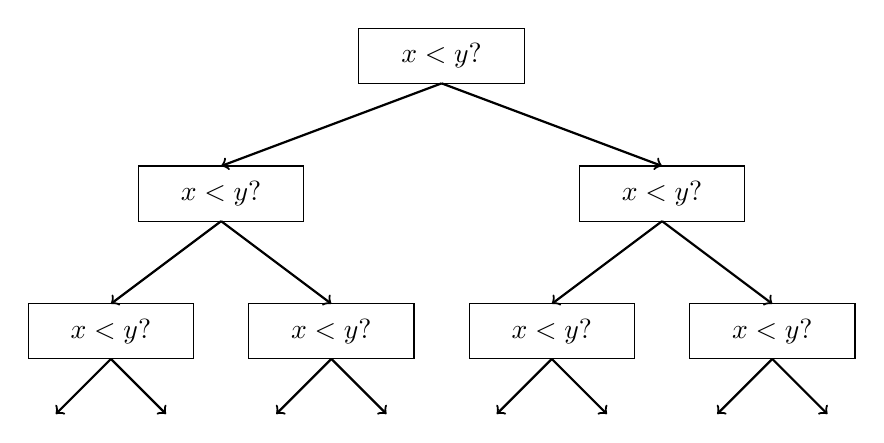
\begin{tikzpicture}[scale=0.7]
\draw (0,0) rectangle (3,1);
\node at (1.5,0.5) {$x < y?$};

\draw[thick,->] (1.5,0) -- (-2.5,-1.5);
\draw[thick,->] (1.5,0) -- (5.5,-1.5);

\draw (-4,-2.5) rectangle (-1,-1.5);
\draw (4,-2.5) rectangle (7,-1.5);
\node at (-2.5,-2) {$x < y?$};
\node at (5.5,-2) {$x < y?$};

\draw[thick,->] (-2.5,-2.5) -- (-4.5,-4);
\draw[thick,->] (-2.5,-2.5) -- (-0.5,-4);
\draw[thick,->] (5.5,-2.5) -- (3.5,-4);
\draw[thick,->] (5.5,-2.5) -- (7.5,-4);

\draw (-6,-5) rectangle (-3,-4);
\draw (-2,-5) rectangle (1,-4);
\draw (2,-5) rectangle (5,-4);
\draw (6,-5) rectangle (9,-4);
\node at (-4.5,-4.5) {$x < y?$};
\node at (-0.5,-4.5) {$x < y?$};
\node at (3.5,-4.5) {$x < y?$};
\node at (7.5,-4.5) {$x < y?$};

\draw[thick,->] (-4.5,-5) -- (-5.5,-6);
\draw[thick,->] (-4.5,-5) -- (-3.5,-6);
\draw[thick,->] (-0.5,-5) -- (0.5,-6);
\draw[thick,->] (-0.5,-5) -- (-1.5,-6);
\draw[thick,->] (3.5,-5) -- (2.5,-6);
\draw[thick,->] (3.5,-5) -- (4.5,-6);
\draw[thick,->] (7.5,-5) -- (6.5,-6);
\draw[thick,->] (7.5,-5) -- (8.5,-6);
\end{tikzpicture}
\end{center}

در اینجا ''$x<y?$'' به معنی مقایسه دو عنصر $x$ و $y$ است.
اگر $x<y$ باشد، فرآیند به سمت چپ ادامه می‌یابد
و در غیر این صورت به سمت راست می‌رود.
نتایج این فرآیند، حالت‌های ممکن برای مرتب‌سازی آرایه هستند
که در مجموع $n!$ حالت است.
به همین دلیل، ارتفاع درخت باید حداقل برابر با مقدار زیر باشد:
\[ \log_2(n!) = \log_2(1)+\log_2(2)+\cdots+\log_2(n).\]
با انتخاب $n/2$ عنصر آخر و تغییر مقدار هر عنصر به $\log_2(n/2)$،
یک کران پایین برای این مجموع به دست می‌آوریم.
این کار تخمین زیر را نتیجه می‌دهد:
\[ \log_2(n!) \ge (n/2) \cdot \log_2(n/2),\]
بنابراین ارتفاع درخت و کمترین تعداد مراحل ممکن در یک الگوریتم مرتب‌سازی
در بدترین حالت، حداقل $n \log n$ است.

\subsubsection{مرتب‌سازی شمارشی}

\index{مرتب‌سازی شمارشی}

کران پایین $n \log n$ برای الگوریتم‌هایی که عناصر آرایه را با یکدیگر مقایسه نمی‌کنند
بلکه از اطلاعات دیگری بهره می‌برند، اعمال نمی‌شود.
یک نمونه از این الگوریتم‌ها \key{مرتب‌سازی شمارشی} است که آرایه را در زمان
$O(n)$ مرتب می‌کند، با این فرض که هر عنصر آرایه
یک عدد صحیح بین $0 \ldots c$ بوده و $c=O(n)$ باشد.

این الگوریتم یک آرایه \emph{شمارش} می‌سازد
که اندیس‌های آن، عناصر آرایه اصلی هستند.
الگوریتم روی آرایه اصلی پیمایش کرده
و تعداد دفعات تکرار هر عنصر در آرایه را محاسبه می‌کند.
\newpage

برای نمونه، آرایه
\begin{center}
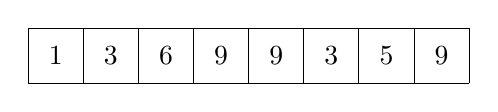
\begin{tikzpicture}[scale=0.7]
\draw (0,0) grid (8,1);
\node at (0.5,0.5) {$1$};
\node at (1.5,0.5) {$3$};
\node at (2.5,0.5) {$6$};
\node at (3.5,0.5) {$9$};
\node at (4.5,0.5) {$9$};
\node at (5.5,0.5) {$3$};
\node at (6.5,0.5) {$5$};
\node at (7.5,0.5) {$9$};
\end{tikzpicture}
\end{center}
متناظر با آرایه شمارش زیر است:
\begin{center}
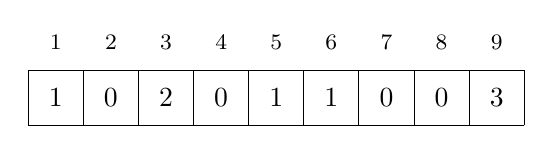
\begin{tikzpicture}[scale=0.7]
\draw (0,0) grid (9,1);
\node at (0.5,0.5) {$1$};
\node at (1.5,0.5) {$0$};
\node at (2.5,0.5) {$2$};
\node at (3.5,0.5) {$0$};
\node at (4.5,0.5) {$1$};
\node at (5.5,0.5) {$1$};
\node at (6.5,0.5) {$0$};
\node at (7.5,0.5) {$0$};
\node at (8.5,0.5) {$3$};

\footnotesize

\node at (0.5,1.5) {$1$};
\node at (1.5,1.5) {$2$};
\node at (2.5,1.5) {$3$};
\node at (3.5,1.5) {$4$};
\node at (4.5,1.5) {$5$};
\node at (5.5,1.5) {$6$};
\node at (6.5,1.5) {$7$};
\node at (7.5,1.5) {$8$};
\node at (8.5,1.5) {$9$};
\end{tikzpicture}
\end{center}

برای مثال، مقدار در موقعیت 3 در آرایه شمارش برابر 2 است،
زیرا عنصر 3 دقیقاً 2 بار در آرایه اصلی آمده است.

ساخت آرایه شمارش زمان $O(n)$ می‌برد. پس از آن،
آرایه مرتب‌شده را می‌توان در زمان $O(n)$ ساخت، زیرا
تعداد رخدادهای هر عنصر از آرایه شمارش قابل بازیابی است.
بنابراین، پیچیدگی زمانی کل مرتب‌سازی شمارشی $O(n)$ است.

مرتب‌سازی شمارشی الگوریتمی بسیار کارآمد است
اما تنها زمانی قابل استفاده است که ثابت $c$ به اندازه کافی کوچک باشد،
به طوری که عناصر آرایه بتوانند به عنوان اندیس در آرایه شمارش به کار روند.

\section{مرتب‌سازی در C++}

\index{sort@\texttt{sort}}

تقریباً هرگز ایده خوبی نیست که در مسابقه
از یک الگوریتم مرتب‌سازی دست‌ساز
استفاده کنید، زیرا پیاده‌سازی‌های خوبی
در زبان‌های برنامه‌نویسی در دسترس است.
برای مثال، کتابخانه استاندارد C++ شامل
تابع \texttt{sort} است که می‌توان از آن به راحتی برای
مرتب‌سازی آرایه‌ها و سایر داده‌ساختارها استفاده کرد.

استفاده از توابع کتابخانه‌ای مزایای زیادی دارد.
نخست، در زمان صرفه‌جویی می‌شود زیرا نیازی به
پیاده‌سازی تابع نیست.
دوم، پیاده‌سازی کتابخانه
قطعاً درست و کارآمد است: بعید است
که یک تابع مرتب‌سازی دست‌ساز عملکرد بهتری داشته باشد.

در این بخش نحوه استفاده از
تابع \texttt{sort} در C++ را بررسی می‌کنیم.
کد زیر یک بردار را
به صورت صعودی مرتب می‌کند:
\begin{lstlisting}
vector<int> v = {4,2,5,3,5,8,3};
sort(v.begin(),v.end());
\end{lstlisting}
پس از مرتب‌سازی، محتویات بردار
به صورت
$[2,3,3,4,5,5,8]$
خواهد بود.
ترتیب پیش‌فرض مرتب‌سازی صعودی است،
اما مرتب‌سازی نزولی نیز به شکل زیر امکان‌پذیر است:
\begin{lstlisting}
sort(v.rbegin(),v.rend());
\end{lstlisting}
یک آرایه معمولی را می‌توان به شکل زیر مرتب کرد:
\begin{lstlisting}
int n = 7; // array size
int a[] = {4,2,5,3,5,8,3};
sort(a,a+n);
\end{lstlisting}
\newpage
کد زیر رشته \texttt{s} را مرتب می‌کند:
\begin{lstlisting}
string s = "monkey";
sort(s.begin(), s.end());
\end{lstlisting}
مرتب‌سازی یک رشته به این معناست که نویسه‌های
آن رشته مرتب می‌شوند.
برای مثال، رشته ''monkey'' تبدیل به ''ekmnoy'' می‌شود.

\subsubsection{عملگرهای مقایسه}

\index{comparison operator}

تابع \texttt{sort} نیازمند آن است که
یک \key{عملگر مقایسه} برای نوع داده
عناصر مورد نظر تعریف شده باشد.
هنگام مرتب‌سازی، هر جا که تعیین ترتیب دو عنصر لازم باشد
از این عملگر استفاده می‌شود.

بیشتر انواع داده C++ عملگر مقایسه توکار دارند
و عناصر این نوع‌ها را می‌توان به صورت خودکار مرتب کرد.
برای مثال، اعداد بر اساس مقادیر عددی‌شان
و رشته‌ها به ترتیب الفبایی مرتب می‌شوند.

\index{pair@\texttt{pair}}

جفت‌ها (\texttt{pair}) در درجه اول بر اساس
عنصر اول (\texttt{first}) مرتب می‌شوند.
با این حال، اگر عنصر اول دو جفت برابر باشد،
بر اساس عنصر دوم (\texttt{second}) مرتب خواهند شد:
\begin{lstlisting}
vector<pair<int,int>> v;
v.push_back({1,5});
v.push_back({2,3});
v.push_back({1,2});
sort(v.begin(), v.end());
\end{lstlisting}
پس از این کار، ترتیب جفت‌ها به صورت
$(1,2)$، $(1,5)$ و $(2,3)$ خواهد بود.

\index{tuple@\texttt{tuple}}

به طور مشابه، چندتایی‌ها (\texttt{tuple})
در درجه اول با عنصر نخست،
سپس با عنصر دوم و الی آخر مرتب می‌شوند\footnote{توجه داشته باشید که در برخی کامپایلرهای قدیمی‌تر،
برای ساخت یک چندتایی باید از تابع \texttt{make\_tuple} به جای
آکولاد استفاده کرد (برای مثال، \texttt{make\_tuple(2,1,4)} به جای \texttt{\{2,1,4\}}).}:
\begin{lstlisting}
vector<tuple<int,int,int>> v;
v.push_back({2,1,4});
v.push_back({1,5,3});
v.push_back({2,1,3});
sort(v.begin(), v.end());
\end{lstlisting}
پس از این کار، ترتیب چندتایی‌ها به صورت
$(1,5,3)$، $(2,1,3)$ و $(2,1,4)$ خواهد بود.

\subsubsection{ساختارهای تعریف‌شده توسط کاربر}

ساختارهای تعریف‌شده توسط کاربر به طور خودکار عملگر مقایسه ندارند.
عملگر باید درون ساختار به عنوان تابع \texttt{operator<} تعریف شود،
که پارامتر آن عنصر دیگری از همان نوع است.
اگر عنصر کوچکتر از پارامتر باشد، عملگر باید \texttt{true} بازگرداند،
و در غیر این صورت \texttt{false}.

برای مثال، ساختار \texttt{P} زیر شامل مختصات x و y یک نقطه است.
عملگر مقایسه طوری تعریف شده است که
نقاط در وهله اول بر اساس مختصات x
و در وهله دوم بر اساس مختصات y مرتب شوند.

\begin{lstlisting}
struct P {
    int x, y;
    bool operator<(const P &p) {
        if (x != p.x) return x < p.x;
        else return y < p.y;
    }
};
\end{lstlisting}

\subsubsection{توابع مقایسه}

\index{comparison function}

همچنین می‌توان یک \key{تابع مقایسه} خارجی را به عنوان تابع بازگشتی (callback)
به تابع \texttt{sort} داد.
برای مثال، تابع مقایسه \texttt{comp} زیر
رشته‌ها را ابتدا بر اساس طول و سپس بر اساس ترتیب الفبایی مرتب می‌کند:

\begin{lstlisting}
bool comp(string a, string b) {
    if (a.size() != b.size()) return a.size() < b.size();
    return a < b;
}
\end{lstlisting}
اکنون برداری از رشته‌ها را می‌توان به صورت زیر مرتب کرد:
\begin{lstlisting}
sort(v.begin(), v.end(), comp);
\end{lstlisting}

\section{جستجوی دودویی}

\index{binary search}

یک روش کلی برای جستجوی عنصر در آرایه،
استفاده از حلقه \texttt{for} است که روی عناصر آرایه پیمایش می‌کند.
برای مثال، کد زیر به دنبال عنصر $x$ در یک آرایه می‌گردد:

\begin{lstlisting}
for (int i = 0; i < n; i++) {
    if (array[i] == x) {
        // x found at index i
    }
}
\end{lstlisting}

پیچیدگی زمانی این رویکرد $O(n)$ است،
زیرا در بدترین حالت، بررسی تمام عناصر آرایه ضروری است.
اگر ترتیب عناصر تصادفی باشد، این بهترین رویکرد ممکن نیز هست،
زیرا اطلاعات اضافه‌ای درباره محل جستجوی عنصر $x$ در دسترس نیست.

اما اگر آرایه \emph{مرتب‌شده} باشد،
اوضاع فرق می‌کند.
در این حالت می‌توان جستجو را بسیار سریع‌تر انجام داد،
زیرا ترتیب عناصر در آرایه، جستجو را هدایت می‌کند.
الگوریتم \key{جستجوی دودویی} زیر
یک عنصر را در آرایه مرتب‌شده در زمان $O(\log n)$ جستجو می‌کند.

\subsubsection{روش ۱}

روش معمول برای پیاده‌سازی جستجوی دودویی
مشابه جستجوی کلمه در فرهنگ لغت است.
جستجو یک محدوده فعال را در آرایه نگه می‌دارد،
که در ابتدا شامل تمام عناصر آرایه است.
سپس مراحلی انجام می‌شود
که هر کدام اندازه محدوده را نصف می‌کنند.

در هر مرحله، عنصر میانی محدوده فعال بررسی می‌شود.
اگر عنصر میانی همان عنصر هدف باشد،
جستجو پایان می‌یابد.
در غیر این صورت، جستجو بسته به مقدار عنصر میانی،
به صورت بازگشتی در نیمه چپ یا راست محدوده ادامه می‌یابد.

ایده بالا این‌گونه پیاده‌سازی می‌شود:
\begin{lstlisting}
int a = 0, b = n-1;
while (a <= b) {
    int k = (a+b)/2;
    if (array[k] == x) {
        // x found at index k
    }
    if (array[k] > x) b = k-1;
    else a = k+1;
}
\end{lstlisting}

در این پیاده‌سازی، ناحیه فعال $a \ldots b$ است
و در ابتدا این ناحیه $0 \ldots n-1$ است.
الگوریتم در هر گام اندازه ناحیه را نصف می‌کند،
بنابراین پیچیدگی زمانی $O(\log n)$ است.

\subsubsection{روش ۲}

روش دیگر برای پیاده‌سازی جستجوی دودویی
مبتنی بر شیوه‌ای کارآمد برای پیمایش عناصر آرایه است.
ایده کار، جهش به جلو و کاهش سرعت جهش هنگام نزدیک شدن به عنصر هدف است.

جستجو در آرایه از چپ به راست حرکت می‌کند،
و طول جهش اولیه $n/2$ است.
در هر گام، طول جهش نصف می‌شود:
ابتدا $n/4$، سپس $n/8$، $n/16$ و غیره، تا اینکه در نهایت طول جهش برابر با ۱ شود.
پس از پایان جهش‌ها، یا عنصر هدف پیدا شده است
یا معلوم می‌شود درون آرایه وجود ندارد.

کد زیر ایده بالا را پیاده‌سازی می‌کند:
\begin{lstlisting}
int k = 0;
for (int b = n/2; b >= 1; b /= 2) {
    while (k+b < n && array[k+b] <= x) k += b;
}
if (array[k] == x) {
    // x found at index k
}
\end{lstlisting}

در طول جستجو، متغیر $b$ طول جهش کنونی را نگه می‌دارد.
پیچیدگی زمانی الگوریتم $O(\log n)$ است،
زیرا کد درون حلقه \texttt{while} برای هر طول جهش حداکثر دو بار اجرا می‌شود.

\subsubsection{توابع ++C}

کتابخانه استاندارد ++C شامل توابع زیر است
که بر پایه جستجوی دودویی بوده و در زمان لگاریتمی عمل می‌کنند:

\begin{itemize}
\item تابع \texttt{lower\_bound} اشاره‌گری به نخستین عنصر آرایه برمی‌گرداند که مقدار آن حداقل $x$ است.
\item تابع \texttt{upper\_bound} اشاره‌گری به نخستین عنصر آرایه برمی‌گرداند که مقدار آن بزرگ‌تر از $x$ است.
\item تابع \texttt{equal\_range} هر دو اشاره‌گر بالا را برمی‌گرداند.
\end{itemize}

این توابع فرض می‌کنند که آرایه مرتب است.
اگر چنین عنصری وجود نداشته باشد، اشاره‌گر به عنصر پس از آخرین عنصر آرایه اشاره می‌کند.
برای نمونه، کد زیر مشخص می‌کند آیا آرایه دارای عنصری با مقدار $x$ هست یا خیر:

\begin{lstlisting}
auto k = lower_bound(array,array+n,x)-array;
if (k < n && array[k] == x) {
    // x found at index k
}
\end{lstlisting}

سپس، کد زیر شمار عناصر دارای مقدار $x$ را به دست می‌آورد:

\begin{lstlisting}
auto a = lower_bound(array, array+n, x);
auto b = upper_bound(array, array+n, x);
cout << b-a << "\n";
\end{lstlisting}

با استفاده از \texttt{equal\_range}، کد کوتاه‌تر می‌شود:

\begin{lstlisting}
auto r = equal_range(array, array+n, x);
cout << r.second-r.first << "\n";
\end{lstlisting}

\subsubsection{یافتن کوچک‌ترین جواب}

کاربرد مهم جستجوی دودویی یافتن نقطه‌ای است که مقدار یک \emph{تابع} در آن تغییر می‌کند. فرض کنید می‌خواهیم کوچک‌ترین مقدار $k$ را بیابیم که جواب معتبری برای مسئله باشد. تابع $\texttt{ok}(x)$ به ما داده شده است که اگر $x$ جوابی معتبر باشد، مقدار \texttt{true} و در غیر این صورت \texttt{false} برمی‌گرداند. همچنین می‌دانیم به ازای $x<k$ مقدار $\texttt{ok}(x)$ برابر \texttt{false} و به ازای $x \ge k$ برابر \texttt{true} است. وضعیت به صورت زیر است:

\begin{center}
\begin{tabular}{r|rrrrrrrr}
$x$ & 0 & 1 & $\cdots$ & $k-1$ & $k$ & $k+1$ & $\cdots$ \\
\hline
$\texttt{ok}(x)$ & \texttt{false} & \texttt{false}
& $\cdots$ & \texttt{false} & \texttt{true} & \texttt{true} & $\cdots$ \\
\end{tabular}
\end{center}

\noindent
اکنون مقدار $k$ با جستجوی دودویی به دست می‌آید:

\begin{lstlisting}
int x = -1;
for (int b = z; b >= 1; b /= 2) {
    while (!ok(x+b)) x += b;
}
int k = x+1;
\end{lstlisting}

این جستجو بزرگ‌ترین مقدار $x$ را می‌یابد که به ازای آن $\texttt{ok}(x)$ برابر \texttt{false} است. در نتیجه مقدار بعدی، یعنی $k=x+1$، کوچک‌ترین مقدار ممکن است که به ازای آن $\texttt{ok}(k)$ برابر \texttt{true} می‌شود. طول پرش اولیه $z$ باید به اندازه کافی بزرگ باشد؛ مثلا مقداری که از قبل می‌دانیم $\texttt{ok}(z)$ برای آن \texttt{true} است.

الگوریتم تابع \texttt{ok} را $O(\log z)$ بار فراخوانی می‌کند، بنابراین پیچیدگی زمانی کل به تابع \texttt{ok} وابسته است. برای نمونه، اگر زمان اجرای این تابع $O(n)$ باشد، پیچیدگی زمانی کل $O(n \log z)$ خواهد بود.

\subsubsection{یافتن بیشینه مقدار}

جستجوی دودویی برای یافتن بیشینه مقدار تابعی که ابتدا صعودی و سپس نزولی است نیز به کار می‌رود. هدف یافتن موقعیت $k$ است به طوری که:

\begin{itemize}
\item
به ازای $x<k$ داشته باشیم $f(x)<f(x+1)$، و
\item
به ازای $x \ge k$ داشته باشیم $f(x)>f(x+1)$.
\end{itemize}

ایده کار استفاده از جستجوی دودویی برای یافتن بزرگ‌ترین مقدار $x$ است که در آن $f(x)<f(x+1)$ باشد. این نتیجه می‌دهد $k=x+1$، زیرا $f(x+1)>f(x+2)$ است. کد زیر جستجو را پیاده‌سازی می‌کند:

\begin{lstlisting}
int x = -1;
for (int b = z; b >= 1; b /= 2) {
    while (f(x+b) < f(x+b+1)) x += b;
}
int k = x+1;
\end{lstlisting}

برخلاف جستجوی دودویی معمولی، اینجا مقادیر متوالی تابع نباید برابر باشند. در صورت برابری، تعیین جهت ادامه جستجو ناممکن می‌شود.